\documentclass{article}

% Numeric, bracketed citations (matches the NeurIPS convention) rather than
% natbib's author-year default — must be set before neurips_2023 loads natbib.
\PassOptionsToPackage{numbers, compress}{natbib}

% Non-anonymous preprint, per NeurIPS 2023 style files:
% https://neurips.cc/Conferences/2023/PaperInformation/StyleFiles
\usepackage[preprint]{neurips_2023}

\usepackage[utf8]{inputenc}
\usepackage[T1]{fontenc}
\usepackage{hyperref}
\usepackage{url}
\usepackage{booktabs}
\usepackage{amsfonts}
\usepackage{amsmath}
\usepackage{nicefrac}
\usepackage{microtype}
\usepackage{xcolor}
\usepackage{graphicx}
\usepackage{caption}
\usepackage{enumitem}

\hypersetup{
    colorlinks=true,
    linkcolor=blue,
    urlcolor=blue,
    citecolor=blue,
    pdftitle={Benchmarking the Evaluators: AST vs. LLM-as-a-Judge},
    pdfauthor={Amit Saxena}
}

\title{Benchmarking the Evaluators: Deterministic AST Parsing vs.\
LLM-as-a-Judge for Structural Technique Detection in Code}

\author{%
  Amit Saxena \\
  Saarland University --- MPI-SWS \\
  \texttt{amsa00003@stud.uni-saarland.de}
}

\begin{document}
\maketitle

\begin{abstract}
Modern adversarial creativity benchmarks for large language models (e.g.\
Denial Prompting) enforce structural code constraints --- ``do not use a
for-loop'' --- but typically verify compliance using \emph{another} LLM as a
judge: a probabilistic check applied to what is fundamentally a deterministic,
binary question. This project quantifies the resulting error empirically. We
parse 4{,}725 real, verified-correct Python solutions from the NeoCoder
competitive-programming dataset with Python's native \texttt{ast} module to
obtain a 100\%-accurate structural ground truth across six technique
categories (for-loops, while-loops, recursion, list comprehensions, lambdas,
sorting calls). We then compare this ground truth against two LLM judges: the
GPT-4 labels already shipped with the dataset (full coverage, $N=4{,}725$) and
a freshly-run, controlled Llama-3.1-8B judge (stratified sample, $N=60$). The
shipped GPT-4 labels achieve a macro-averaged F1 of only 0.50 --- including a
100\% miss rate on two technique categories and a 47\% hallucination rate on
the most common one. A freshly-prompted judge performs far better
(F1~$\approx$~0.97) but is still not error-free. A complementary embedding
analysis (DeBERTa-v3-large) shows that semantic similarity between
same-problem solution pairs explains only $\approx$5\% of the variance in
their structural similarity (Pearson $r = 0.227$). We conclude that
rule-bound code-creativity evaluation requires a \emph{dual-axis} approach ---
deterministic AST parsing for structural constraints, alongside semantic
embeddings for functional equivalence --- rather than an LLM judge alone.
\end{abstract}

\tableofcontents

% ============================================================
\section{Introduction and Motivation}
% ============================================================

Adversarial creativity benchmarks increasingly evaluate large language models
by imposing algorithmic constraints on the code they generate --- forbidding a
\texttt{for} loop, requiring recursion instead of iteration, and so on --- in
order to force divergent, out-of-the-box solutions and counteract mode
collapse. To check whether a generated solution actually obeys such a
constraint, these benchmarks overwhelmingly rely on an \textbf{LLM-as-a-Judge}
architecture: a second language model reads the generated code and reports
which techniques it used.

This is a methodological gamble. Verifying ``does this code contain a
\texttt{for} loop'' is not a matter of judgment or interpretation --- it is a
deterministic fact about the code's grammar, answerable with 100\% certainty
by parsing the code into an Abstract Syntax Tree (AST). Using a probabilistic,
sampling-based text generator to answer a question that already has an exact
mechanical answer introduces an unmeasured, unnecessary source of error into
what should be a completely reliable check.

This project's core question is therefore simple to state and expensive to
verify at scale: \emph{how large is that error, in practice, on real code?}
Rather than argue in the abstract, we build a full empirical pipeline that
parses thousands of real, verified-correct human solutions with a
deterministic AST visitor, and directly measures how often two different LLM
judges --- one already embedded in a widely-used benchmark, one freshly
controlled by us --- agree or disagree with that ground truth.

We additionally test a natural counter-argument: that semantic code embeddings
(e.g.\ DeBERTa) might already capture enough information to substitute for
structural parsing, since two solutions that are highly similar in embedding
space are often assumed to be ``basically the same solution.'' We show this
assumption does not hold for structural compliance, even restricted to the
strongest possible test case: two solutions to the \emph{exact same} problem.

% ============================================================
\section{Methodology (Starting Process)}
% ============================================================

\subsection{Dataset}

We use the \textbf{NeoCoder} dataset~\citep{neocoder} (Codeforces human solutions), which
ships $5{,}970$ human-written solutions across 199 competitive-programming
problems, spanning multiple programming languages, along with a pre-computed
set of technique labels generated by GPT-4 for each solution. Since our
ground-truth mechanism (Python's \texttt{ast} module) is Python-specific, we
filter the dataset to Python-parseable solutions only, retaining
\textbf{4{,}725 solutions across 198 problems}. No information is lost for the
structural analysis --- the filtered set is simply the subset the
deterministic parser can operate on.

\subsection{Techniques Evaluated}

We selected six atomic, unambiguously-detectable structural techniques, each
directly identifiable via a single AST node type or call pattern:

\begin{center}
\begin{tabular}{lp{8cm}}
\toprule
\textbf{Technique} & \textbf{AST detection rule} \\
\midrule
\texttt{for\_loop} & any \texttt{ast.For} node \\
\texttt{while\_loop} & any \texttt{ast.While} node \\
\texttt{recursion} & a function that calls itself (bare or \texttt{self.}/\texttt{obj.}-qualified) \\
\texttt{list\_comprehension} & any \texttt{ast.ListComp} node \\
\texttt{lambda} & any \texttt{ast.Lambda} node \\
\texttt{sorting} & a call to \texttt{sorted()} or a \texttt{.sort()} method \\
\bottomrule
\end{tabular}
\end{center}

\subsection{Pipeline}

The full analysis runs as a five-phase pipeline:

\begin{enumerate}[label=\textbf{Phase \arabic*.}, leftmargin=2.2cm]
\item \textbf{Data ingestion.} Download and cache the NeoCoder solution and
  label files; filter to Python-parseable solutions.
\item \textbf{Deterministic AST ground truth.} A \texttt{TechniqueVisitor}
  subclassing Python's \texttt{ast.NodeVisitor} traverses every solution once
  and produces a binary label vector over the six techniques. This is, by
  construction, 100\% accurate --- it is a direct read of the language
  grammar, not an inference.
\item \textbf{LLM-as-a-Judge evaluation}, in two independent variants:
  \begin{itemize}
    \item \emph{GPT-4 labels}: the technique labels already shipped with the
      NeoCoder dataset, converted into the same binary format as the AST
      labels. Full coverage ($N = 4{,}725$), no additional API calls.
    \item \emph{Live Llama-3.1-8B-Instant judge}: each solution is sent,
      individually, to Llama-3.1-8B~\citep{llama3} via the Groq
      API~\citep{groq} with a fixed prompt
      asking which of the six techniques are present. Due to free-tier
      rate limits, this is run on a \emph{stratified} sample of 60
      solutions, deliberately chosen so every technique --- including rare
      ones such as \texttt{lambda} and \texttt{recursion} --- is represented,
      rather than a random sample that would be $\sim$95\% \texttt{for\_loop}.
  \end{itemize}
\item \textbf{Embedding vs.\ structure analysis.} Solutions are encoded with
  \texttt{microsoft/deberta-v3-large}~\citep{deberta} (mean-pooled last hidden state). For
  pairs of solutions to the \emph{same} problem --- the only pairs guaranteed
  functionally equivalent, since they all pass that problem's test suite ---
  we compute both the cosine similarity of their embeddings (semantic
  similarity) and the Jaccard similarity of their AST technique sets
  (structural similarity), and correlate the two.
\item \textbf{Reporting.} Per-technique accuracy / precision / recall / F1 /
  false-positive-rate / false-negative-rate are computed for both LLM judges
  against the AST ground truth, alongside a problem-level ``creativity-score
  impact'' analysis (Section~\ref{sec:results}.4).
\end{enumerate}

% ============================================================
\section{Results}
\label{sec:results}
% ============================================================

Throughout this section: \textbf{FPR} (false-positive rate) is the
\emph{hallucination rate} --- the judge reports a technique that is not
actually present. \textbf{FNR} (false-negative rate) is the \emph{miss rate}
--- the judge fails to detect a technique that is present. \textbf{Accuracy}
alone is misleading here due to class imbalance (Section~\ref{sec:prevalence}),
so F1 (the harmonic mean of precision and recall) is the more reliable
single-number summary.

\subsection{AST Ground Truth --- Technique Prevalence}
\label{sec:prevalence}

\begin{center}
\begin{tabular}{lrrr}
\toprule
\textbf{Technique} & \textbf{Positive} & \textbf{Total} & \textbf{Prevalence} \\
\midrule
\texttt{for\_loop}           & 4{,}505 & 4{,}725 & 95.3\% \\
\texttt{while\_loop}         & 480     & 4{,}725 & 10.2\% \\
\texttt{recursion}           & 3       & 4{,}725 & 0.1\%  \\
\texttt{list\_comprehension} & 514     & 4{,}725 & 10.9\% \\
\texttt{lambda}              & 137     & 4{,}725 & 2.9\%  \\
\texttt{sorting}             & 548     & 4{,}725 & 11.6\% \\
\bottomrule
\end{tabular}
\end{center}

\texttt{for\_loop} dominates the dataset (95.3\% of solutions), while
\texttt{recursion} is almost never used (3 solutions total). \emph{Small-sample
caveat:} with only 3 ground-truth positives, precision/recall/F1 for
\texttt{recursion} in the tables below are highly sensitive to individual
misclassifications and should be read as directional rather than precise.

\subsection{LLM Judge Error Rates vs.\ AST Ground Truth}

\subsubsection{Llama-3.1-8B-Instant (live run, stratified sample)}

\begin{center}
\begin{tabular}{lrrrrrrr}
\toprule
\textbf{Technique} & \textbf{Acc.} & \textbf{Prec.} & \textbf{Recall} & \textbf{F1} & \textbf{FPR} & \textbf{FNR} & \textbf{N} \\
\midrule
\texttt{for\_loop}           & 0.950 & 0.965 & 0.982 & 0.974 & 0.500 & 0.018 & 60 \\
\texttt{while\_loop}         & 1.000 & 1.000 & 1.000 & 1.000 & 0.000 & 0.000 & 60 \\
\texttt{recursion}           & 1.000 & 1.000 & 1.000 & 1.000 & 0.000 & 0.000 & 60 \\
\texttt{list\_comprehension} & 0.950 & 0.833 & 1.000 & 0.909 & 0.067 & 0.000 & 60 \\
\texttt{lambda}              & 1.000 & 1.000 & 1.000 & 1.000 & 0.000 & 0.000 & 60 \\
\texttt{sorting}             & 0.983 & 0.923 & 1.000 & 0.960 & 0.021 & 0.000 & 60 \\
\midrule
\textbf{Macro avg} & \textbf{0.981} & \textbf{0.954} & \textbf{0.997} & \textbf{0.974} & \textbf{0.098} & \textbf{0.003} & --- \\
\bottomrule
\end{tabular}
\end{center}

A carefully-prompted, freshly-run judge performs very well overall
(macro F1~$\approx$~0.97) --- but is still not perfect: it hallucinates
\texttt{for\_loop} in 50\% of the (few) cases where a for-loop is genuinely
absent, and \texttt{list\_comprehension} in 6.7\% of cases.

\subsubsection{GPT-4 (pre-computed labels shipped with NeoCoder, full coverage)}

\begin{center}
\begin{tabular}{lrrrrrrr}
\toprule
\textbf{Technique} & \textbf{Acc.} & \textbf{Prec.} & \textbf{Recall} & \textbf{F1} & \textbf{FPR} & \textbf{FNR} & \textbf{N} \\
\midrule
\texttt{for\_loop}           & 0.976 & 0.978 & 0.998 & 0.988 & 0.468 & 0.002 & 4{,}725 \\
\texttt{while\_loop}         & 0.987 & 0.998 & 0.875 & 0.932 & 0.000 & 0.125 & 4{,}725 \\
\texttt{recursion}           & 0.998 & 0.182 & 0.667 & 0.286 & 0.002 & 0.333 & 4{,}725 \\
\texttt{list\_comprehension} & 0.891 & 0.000 & 0.000 & 0.000 & 0.000 & 1.000 & 4{,}725 \\
\texttt{lambda}              & 0.971 & 0.000 & 0.000 & 0.000 & 0.000 & 1.000 & 4{,}725 \\
\texttt{sorting}             & 0.962 & 0.984 & 0.679 & 0.803 & 0.001 & 0.321 & 4{,}725 \\
\midrule
\textbf{Macro avg} & \textbf{0.964} & \textbf{0.524} & \textbf{0.536} & \textbf{0.502} & \textbf{0.079} & \textbf{0.464} & --- \\
\bottomrule
\end{tabular}
\end{center}

These are the labels a real adversarial-creativity benchmark would actually
depend on today. 96.4\% accuracy looks strong until class imbalance is
accounted for: macro-averaged F1 is only \textbf{0.50}. \texttt{for\_loop} ---
the one technique the labeling process clearly does track --- is
\emph{hallucinated} 46.8\% of the time it is absent, a genuine, live judgment
error.

\paragraph{Vocabulary-gap caveat.} Neither \texttt{lambda} nor
\texttt{list\_comprehension} ever appears, as a string, anywhere in the raw
GPT-4 label vocabulary shipped with the dataset (0 occurrences across every
unique technique label, any problem, any language, out of 41 total unique
label strings observed). Their 100\% miss rate (FNR~$=1.0$) is therefore best
explained as a \textbf{taxonomy gap} --- the process that generated these
labels apparently never offered these two categories as options --- rather
than GPT-4 examining a lambda expression and failing to recognize it. This is
a different, and arguably more damning, failure mode than \texttt{for\_loop}'s
hallucination rate: it means the benchmark's underlying label taxonomy is
structurally incomplete, not merely imprecise.

\subsection{Embedding vs.\ Structure Analysis}

\begin{center}
\textbf{Pearson $r$} (cosine similarity vs.\ structural Jaccard similarity,
\emph{same-problem pairs only}): $\mathbf{r = 0.227}$
(95\% CI: $[0.201,\ 0.253]$, $n = 5{,}000$ pairs)
\end{center}

Pairs are restricted to two solutions of the \emph{same} problem --- the only
pairs guaranteed functionally equivalent, since every human solution to a
given problem passed that problem's test suite. This correlation is small but,
given the tight confidence interval, statistically distinguishable from zero:
the two axes are \emph{not} strictly orthogonal. However, $r^2 \approx 5.2\%$
means semantic similarity explains only about 5\% of the variance in
structural similarity --- the vast majority of whether two functionally
equivalent solutions share the same structural techniques remains invisible
to embeddings alone.

\begin{figure}[htbp]
  \centering
  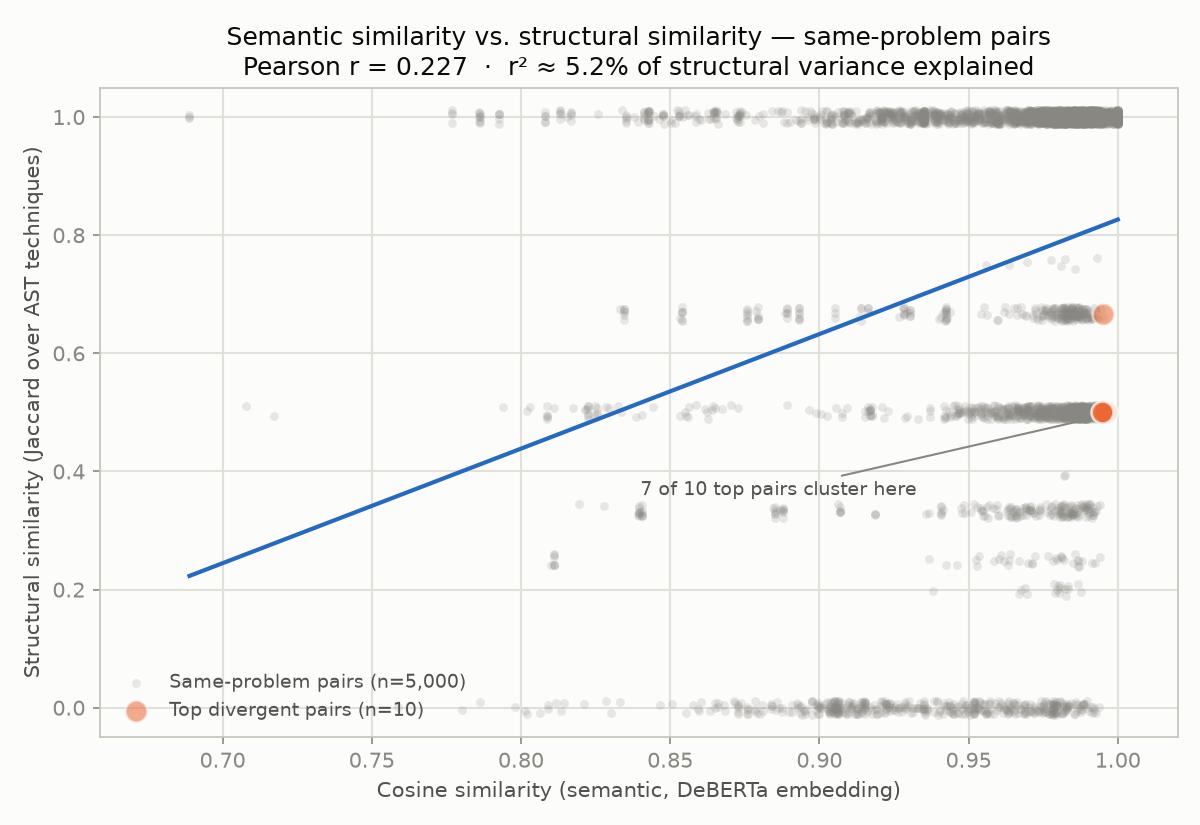
\includegraphics[width=0.85\textwidth]{figures/embedding_scatter.png}
  \caption{Cosine similarity (semantic, DeBERTa embedding) vs.\ structural
  similarity (Jaccard over AST techniques) for 5{,}000 same-problem solution
  pairs. The shallow trend-line slope is the visual counterpart of
  $r^2 \approx 5.2\%$. Highlighted points: the ten most striking cases where
  two solutions to the identical problem are $>$99\% similar by embedding yet
  differ in a structural technique.}
  \label{fig:embedding-scatter}
\end{figure}

\subsubsection{Top Divergent Pairs}

Table~\ref{tab:divergent} lists the ten pairs with the highest cosine
similarity that nonetheless differ in AST-detected technique. Every pair is
two solutions to the \emph{same} problem, so functional equivalence is
guaranteed by construction --- yet the embedding model rates them
near-identical while the structural check finds a clear difference.

\begin{table}[htbp]
\centering
\begin{tabular}{clcc}
\toprule
\textbf{\#} & \textbf{Problem} & \textbf{Cosine Sim.} & \textbf{Differing Technique} \\
\midrule
1  & 1859A & 0.996 & \texttt{sorting} \\
2  & 1747A & 0.996 & \texttt{sorting} \\
3  & 1747A & 0.996 & \texttt{list\_comprehension} \\
4  & 1747A & 0.996 & \texttt{list\_comprehension} \\
5  & 1747A & 0.996 & \texttt{sorting} \\
6  & 1733A & 0.995 & \texttt{list\_comprehension} \\
7  & 1873B & 0.995 & \texttt{sorting} \\
8  & 1734A & 0.995 & \texttt{list\_comprehension} \\
9  & 1873B & 0.995 & \texttt{sorting} \\
10 & 1873B & 0.995 & \texttt{sorting} \\
\bottomrule
\end{tabular}
\caption{Top divergent same-problem pairs: near-identical embeddings, differing structure.}
\label{tab:divergent}
\end{table}

\subsection{LLM Error Impact on Historical Creativity Scores}

The proposal's central practical claim is that LLM-as-a-Judge errors propagate
into \emph{problem-level diversity assessments} --- the kind of ``creativity
score'' used by benchmarks such as Denial Prompting. For each problem, we
check whether the judge correctly identifies which techniques are present in
\emph{at least one} solution to that problem.

\begin{center}
\begin{tabular}{lrrrrr}
\toprule
\textbf{Technique} & \textbf{Correct} & \textbf{Inflated} & \textbf{Deflated} & \textbf{Total} & \textbf{Error Rate} \\
\midrule
\multicolumn{6}{l}{\emph{Llama-3.1-8B-Instant (stratified sample)}} \\
\texttt{for\_loop}           & 14 & 1 & 1 & 16 & 12.5\% \\
\texttt{while\_loop}         & 16 & 0 & 0 & 16 & 0.0\%  \\
\texttt{recursion}           & 16 & 0 & 0 & 16 & 0.0\%  \\
\texttt{list\_comprehension} & 15 & 1 & 0 & 16 & 6.2\%  \\
\texttt{lambda}              & 16 & 0 & 0 & 16 & 0.0\%  \\
\texttt{sorting}             & 16 & 0 & 0 & 16 & 0.0\%  \\
\textbf{Macro avg} & & & & & \textbf{3.1\%} \\
\midrule
\multicolumn{6}{l}{\emph{GPT-4 (full coverage)}} \\
\texttt{for\_loop}           & 197 & 1 & 0   & 198 & 0.5\%  \\
\texttt{while\_loop}         & 190 & 1 & 7   & 198 & 4.0\%  \\
\texttt{recursion}           & 189 & 8 & 1   & 198 & 4.5\%  \\
\texttt{list\_comprehension} & 51  & 0 & 147 & 198 & 74.2\% \\
\texttt{lambda}              & 128 & 0 & 70  & 198 & 35.4\% \\
\texttt{sorting}             & 189 & 3 & 6   & 198 & 4.5\%  \\
\textbf{Macro avg} & & & & & \textbf{20.5\%} \\
\bottomrule
\end{tabular}
\end{center}

\emph{Inflated} = the judge reports a technique present when AST shows it
absent (hallucination propagates into an inflated diversity score).
\emph{Deflated} = AST shows the technique present but the judge missed it
(under-reporting deflates the diversity score).

Using GPT-4's shipped labels, approximately \textbf{20.5\% of all
problem-level technique-diversity assessments are incorrect} --- rising to
\textbf{74.2\%} for \texttt{list\_comprehension} specifically --- directly
quantifying the epistemological error a real benchmark inherits by relying on
these labels. The freshly-run Llama judge is far more reliable at the
problem level (3.1\% error), though measured on a much smaller sample.

\begin{figure}[htbp]
  \centering
  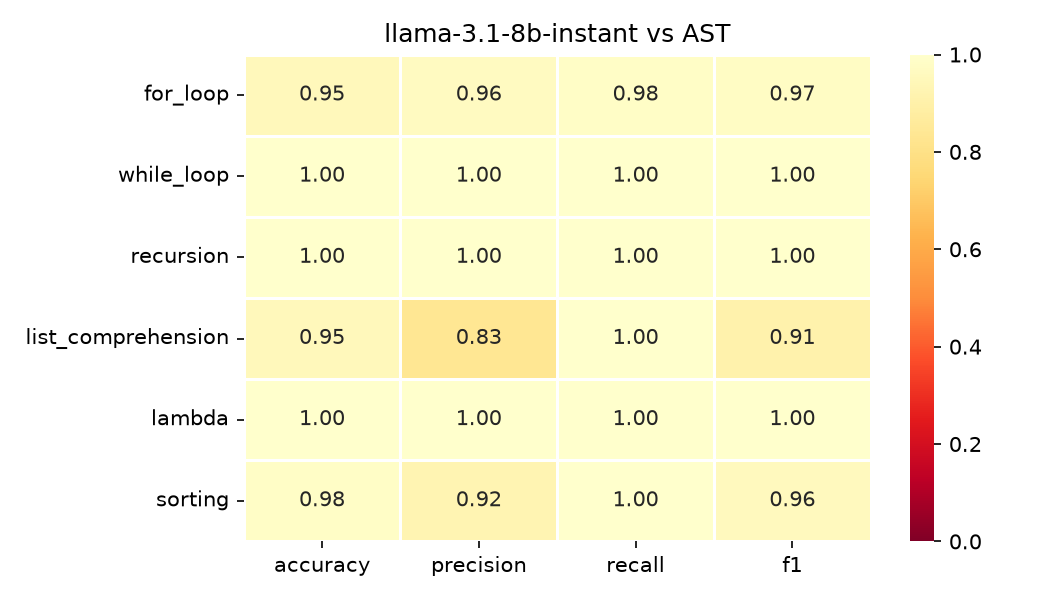
\includegraphics[width=0.75\textwidth]{figures/llm_heatmap.png}
  \caption{Llama-3.1-8B-Instant vs.\ AST ground truth: per-technique accuracy, precision, recall, F1.}
  \label{fig:llm-heatmap}
\end{figure}

\begin{figure}[htbp]
  \centering
  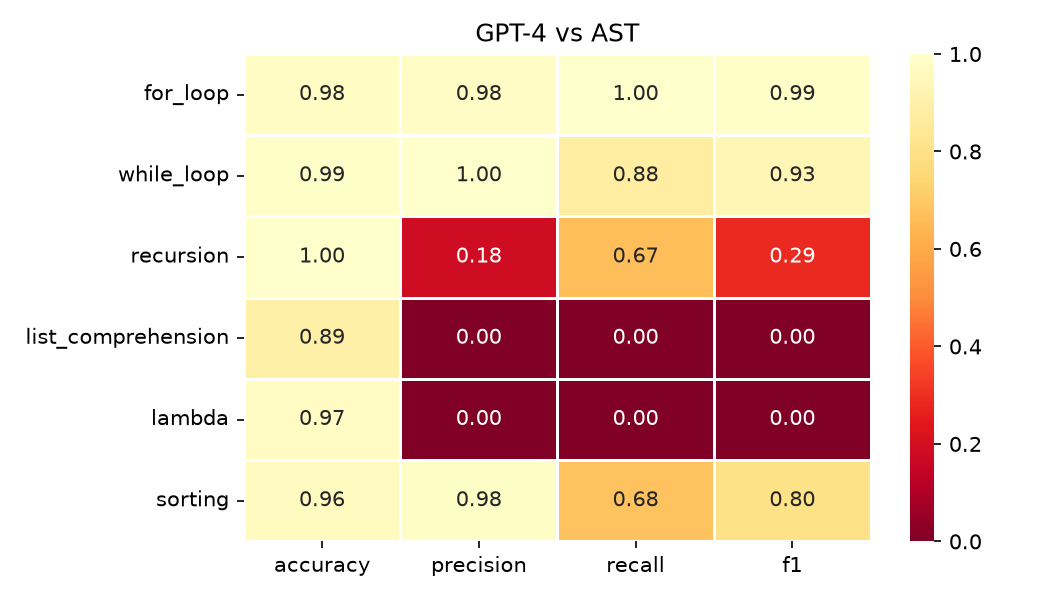
\includegraphics[width=0.75\textwidth]{figures/gpt4_heatmap.png}
  \caption{GPT-4 (shipped labels) vs.\ AST ground truth: per-technique accuracy, precision, recall, F1. Dark cells at F1~=~0 for \texttt{lambda} and \texttt{list\_comprehension} are the vocabulary-gap failure; the high FPR band for \texttt{for\_loop} is a live hallucination.}
  \label{fig:gpt4-heatmap}
\end{figure}

% ============================================================
\section{Discussion and Conclusion}
% ============================================================

Deterministic AST parsing establishes a 100\%-accurate structural ground
truth --- zero error by construction --- against which both LLM judges reveal
measurable, non-zero error.

\textbf{Primary evidence: the GPT-4 labels actually embedded in the
benchmark.} These are the labels real adversarial-creativity frameworks
(NeoCoder, Denial Prompting) depend on today. Measured against AST ground
truth over all 4{,}725 solutions, they show catastrophic, systematic blind
spots: a 100\% miss rate on both \texttt{lambda} and
\texttt{list\_comprehension} (a taxonomy gap, not a live per-solution
failure), and a 47\% hallucination rate on \texttt{for\_loop} (which \emph{is}
a live judgment error, since that category is squarely within the labels'
vocabulary). At the problem level this compounds to a 20.5\%
diversity-assessment error rate, reaching 74\% for individual techniques.

\textbf{Corroborating evidence: a controlled, live judge.} A well-prompted
Llama-3.1-8B-Instant run, evaluated per-solution on a stratified sample,
performs far better (macro F1~$\approx$~0.97) but is still not error-free ---
it hallucinates \texttt{list\_comprehension} and \texttt{for\_loop} at
non-trivial rates. The lesson is that LLM-judge reliability is highly
sensitive to prompt and setup, and no configuration reaches the determinism a
structural constraint demands.

\textbf{Embeddings are not a substitute.} Even restricted to same-problem
pairs --- the strongest possible test of functional equivalence --- the
correlation between semantic similarity and structural compliance is small
($r=0.227$, $r^2\approx5\%$). Semantic similarity is not a reliable proxy for
structural compliance and cannot substitute for deterministic AST parsing
when the constraint being enforced is structural rather than functional.

\textbf{Therefore:} automated creativity evaluation in rule-bound domains
requires a \emph{dual-axis approach} --- deterministic AST parsing to enforce
structural constraints, alongside semantic embeddings for functional
equivalence. Relying on an LLM-as-a-Judge alone introduces an unmeasured,
prompt-dependent error rate into what should be a deterministic mathematical
evaluation.

% ============================================================
\section{Challenges}
% ============================================================

\begin{itemize}[leftmargin=*]

\item \textbf{Free-tier API rate limits.} Groq's free tier caps throughput at
  roughly 6{,}000 tokens/minute, which made evaluating all 4{,}725 solutions
  with the live Llama judge impractical within the project timeline. This was
  addressed by evaluating a \emph{stratified} sample of 60 solutions,
  deliberately enriched with rare techniques, so the judge's failure modes on
  \texttt{lambda}, \texttt{recursion}, and \texttt{list\_comprehension} remain
  measurable rather than being masked by the dominance of \texttt{for\_loop}.

\item \textbf{Model deprecation mid-project.} The Groq-hosted model named in
  the original plan (\texttt{llama3-8b-8192}) was decommissioned during the
  project. It was replaced with the current equivalent-scale successor,
  \texttt{llama-3.1-8b-instant}.

\item \textbf{Dataset heterogeneity.} NeoCoder is multi-language, but AST
  parsing is inherently Python-specific. Solutions had to be filtered to
  Python-parseable code before ground-truth labeling, reducing the usable set
  from 5{,}970 to 4{,}725 solutions.

\item \textbf{Class imbalance and small-sample statistics.} \texttt{for\_loop}
  dominates the dataset (95.3\%), which makes raw accuracy a misleading
  headline metric; F1 and FPR/FNR were used instead. \texttt{recursion} has
  only 3 ground-truth positive examples in the entire dataset, making its
  precision/recall/F1 statistically fragile and requiring an explicit
  small-sample caveat in the report.

\item \textbf{A latent software defect in the ground-truth pipeline.} During
  a later refactor of the AST visitor (switching from \texttt{ast.walk} to
  \texttt{ast.NodeVisitor} to match the original proposal's stated API), an
  unrelated variable-scoping bug was introduced that caused the pipeline to
  crash on any fresh run that was not served from a cached label file. This
  was caught, root-caused, fixed, and verified by re-running the full
  pipeline from a clean state and confirming byte-for-byte-consistent output
  against the previously cached results.

\item \textbf{A methodological flaw in the embedding-pair sampling.} An
  earlier version of the embedding analysis sampled pairs uniformly at random
  from the entire encoded pool, which meant most sampled pairs compared
  solutions to \emph{different} problems --- pairs with no a-priori reason to
  be functionally equivalent, and therefore not a valid test of the
  proposal's claim (which is specifically about same-problem pairs). This was
  identified by manually inspecting the ``top divergent pairs'' output and
  noticing they referenced unrelated problem IDs. The sampling was corrected
  to draw only from same-problem pairs, which changed the measured
  correlation from $r \approx 0.00$ (across unrelated problems) to
  $r = 0.227$ (among genuinely functionally-equivalent solutions) --- a more
  scientifically honest and defensible result.

\item \textbf{Correctly characterizing an LLM failure mode.} Distinguishing
  ``the judge examined the code and got it wrong'' from ``the judge's label
  taxonomy never included this category'' required directly inspecting the
  raw label vocabulary in the dataset, not just the aggregate error metrics.
  This changed how the \texttt{lambda}/\texttt{list\_comprehension} result is
  reported (Section~\ref{sec:results}.2).

\item \textbf{Local compute constraints.} Development was carried out on an
  8\,GB Apple M1 machine. Running the $\sim$8-billion-parameter Llama model
  locally (as an alternative to the Groq API) was evaluated and found
  impractical on this hardware: even quantized, an 8B model leaves very
  little memory headroom, and autoregressive generation is estimated at
  roughly an order of magnitude slower per solution than the equivalent Groq
  API call, despite the API's rate-limit pacing. The much smaller DeBERTa
  embedding model, by contrast, was successfully accelerated using PyTorch's
  Metal (MPS) backend, reducing the embedding phase from
  $\sim$9--10 minutes to roughly 1--1.5 minutes on the same machine.

\end{itemize}

% ============================================================
\section{Deviations from the Original Proposal}
% ============================================================

The implementation departs from the original project proposal in several
places, driven by practical constraints and by what the data empirically
showed. None of these deviations alter the project's core thesis.

\begin{center}
\small
\begin{tabular}{p{0.4cm}p{2.3cm}p{3.2cm}p{3.2cm}p{2.9cm}}
\toprule
\textbf{\#} & \textbf{Area} & \textbf{Proposal said} & \textbf{Implementation does} & \textbf{Reason} \\
\midrule
1 & Dataset size & 5{,}970 solutions / 199 problems & 4{,}725 Python solutions / 198 problems & AST parsing is Python-specific; non-Python solutions filtered out \\
2 & LLM coverage & Feed all $\sim$5.9K solutions to Llama & Stratified sample of 60 solutions & Groq free-tier rate limit \\
3 & LLM sampling & Unspecified & Stratified across techniques & Random sampling masks rare-technique failures \\
4 & Narrative emphasis & Llama as primary LLM judge & GPT-4 (benchmark labels) as primary evidence & Empirical result: GPT-4's shipped labels show the more dramatic, benchmark-relevant failures \\
5 & Llama model & \texttt{Llama-3-8B-Instruct} & \texttt{llama-3.1-8b-instant} & Original Groq model was decommissioned \\
6 & AST traversal & \texttt{ast.NodeVisitor} & \texttt{ast.NodeVisitor} (now matches) & Initially used \texttt{ast.walk}; refactored to match proposal \\
7 & Embedding pair sampling & Unspecified & Restricted to same-problem pairs & Cross-problem pairs are not functionally equivalent and don't test the proposal's claim \\
8 & GPT-4 miss-rate framing & Unspecified & Framed as a labeling-taxonomy gap, not a live LLM miss & Neither \texttt{lambda} nor \texttt{list\_comprehension} ever appears in GPT-4's label vocabulary for this dataset \\
\bottomrule
\end{tabular}
\end{center}

What did \emph{not} change: the core thesis that deterministic AST parsing
provides an infallible ground truth to audit LLM-as-a-Judge frameworks; the
four-phase analytical structure (ground truth $\rightarrow$ LLM error
quantification $\rightarrow$ embedding-vs-structure analysis $\rightarrow$
reporting); the embedding model choice (\texttt{microsoft/deberta-v3-large})
and the orthogonality hypothesis it was used to test; and the final
recommendation that rule-bound creativity benchmarks require a dual-axis
(AST + embeddings) evaluation strategy.

% ============================================================
\section{Code and Data Availability}
% ============================================================

The full implementation --- data ingestion, the deterministic AST visitor,
both LLM-judge integrations, the embedding analysis, and the reporting
pipeline that generates every table and figure in this report --- is
available at:

\begin{center}
\url{https://github.com/amitsaxena-softdev/ast-llm-benchmark}
\end{center}

The repository includes a \texttt{DEVIATIONS.md} file documenting the changes
listed in Section~5 in full detail, and a \texttt{README.md} with setup and
reproduction instructions. The pipeline is fully reproducible via
\texttt{uv run python main.py} (optionally with \texttt{-{}-skip-llm} to avoid
live API calls and reuse the shipped GPT-4 labels instead).

% ============================================================
% thebibliography auto-generates its own "References" heading (via \refname)
% ============================================================

{
\small

\begin{thebibliography}{9}

\bibitem{neocoder}
JHU-CLSP.
\textit{NeoCoder: Codeforces human-solution dataset with technique
annotations.}
GitHub repository.
\url{https://github.com/JHU-CLSP/NeoCoder}

\bibitem{deberta}
Pengcheng He, Jianfeng Gao, and Weizhu Chen.
\textit{DeBERTaV3: Improving DeBERTa using ELECTRA-Style Pre-Training with
Gradient-Disentangled Embedding Sharing.}
arXiv:2111.09543, 2021.

\bibitem{llama3}
Aaron Grattafiori et al.\ (AI@Meta).
\textit{The Llama 3 Herd of Models.}
arXiv:2407.21783, 2024.

\bibitem{groq}
Groq, Inc.
\textit{GroqCloud: Low-latency LPU-based inference API.}
\url{https://groq.com}

\end{thebibliography}
}

\end{document}
